\chapter{Design iteration I}
\label{DesignIteration1}

\begin{flushright}{\slshape    
I think the only way forward is going from applying algorithms to\\
individual transactions, to first placing information in \\
context --- pixels to pictures --- and only applying algorithms \\
after one sees how the transaction relates to the other data.\\
It's the only way that I can see that it's going to close this\\
 sense-making gap.} \\ \medskip
    --- Jeff Jones \cite{AlexWoodie}
\end{flushright}


\marginpar{Parts of this chapter appear in \cite{Niezen2010} and \cite{VanderVlist2010}.}

An iterative development process was followed for the work described in this thesis. In the following chapters three iterations, each consisting of a requirements and planning phase, analysis and design phase, implementation phase and evaluation phase, is described in more detail. Iterative processes are essential to modern-day software and hardware development methodologies, exemplified by the various agile development frameworks \cite{Larman2003}.

\section{Requirements}

Scenarios are commonly used in software engineering and interaction design to help discover and analyse requirements. The following scenario was presented at the start of the project to guide the design process:

\emph{Mark is a 12-year-old boy and he is at home receiving his friend Dries from school. Dries arrives with a portable music player loaded with his favourite songs. He wants to play some recent collections for Mark. Mark's home is equipped with a sophisticated surround sound system, and they have recently installed an ambient lighting system that is connected to the sound system and renders the mood of the music by dynamic colour lighting in the room. They decide to use both to enjoy the music. Dries starts streaming his music to the environment.}

\emph{An object (or several objects) shows possible input and output ports for streaming music in the environment. By interaction with the object/objects, Mark connects the output from Dries' music stream to the input of the sound system. Now the room is full with Dries' music and the colourful lighting effects. Mark's mom, Sofia, now comes back from work. She starts preparing dinner for the family. Mark and Dries don't want to bother her with their loud music. They again use the object(s) to re-arrange the music stream. Now the music is streamed to Mark's portable music player while playing back at Dries'. It is also connected to the ambient lighting system directly, bypassing the sound system. They both are enjoying the same music using their own favourite earphones, and the colourful lighting effects, but without loud music in the environment.}

\emph{The object(s) shows the connection possibilities with a high level of semantic abstraction, hiding the complexity of wired or wireless networks. By interacting with the object(s), semantic connections can be built, redirected, cut or bypassed.}

The first takeaway from this scenario is that the focus is on the connections between the devices, instead of on the devices themselves. This brings us to the first design decision: \emph{Semantic connections} are introduced as a means for users to indicate their intentions concerning the information exchange between smart objects in a smart environment. 


\begin{description}
	\item [Semantic Connection] A semantic connection is a relationship between two entities in a smart environment and focuses on the semantics---or meaning---of the connections between these entities. 
\end{description}

The term semantic connections is used to refer to meaningful connections and relationships between entities in a smart environment. These connections are both real ``physical'' connections (e.g. wired or wireless connections that exist in the real world) and ``mental'' conceptual connections that seem to be there from the user's perspective. The context of the connections, for example the objects that they connect, provide meaning to the connections. The term ``semantics'' refers to the meaningfulness of the connections. The type of connection, which often has the emphasis now (e.g. WiFi, Bluetooth or USB) is not considered to be the most relevant, but what the connection can do for someone --- its functionality --- even more.

%end S3E
The following requirements were defined during this phase:

\begin{itemize}
	\item Semantic connections exist in both the physical and the digital world. We need ways to visualise these invisible connections and to control them. 
	\item Devices need to be able to share their capabilities and content with the other devices in their environment.
\end{itemize}

A number of different approaches to visualising and controlling semantic connections were explored in the first iteration, and these are described in Section \ref{DeviceDesign1}. We also need a way to model the devices, their capabilities and the connections themselves. This is the subject of the next section.



% ``Mark is relaxing at home when his friend Dries arrives. Dries comes with a portable music player loaded with his favourite songs. He wants to play some of his recent collections for Mark. Mark's home is equipped with a sophisticated surround sound system. They decide to enjoy the music from the music player on the sound system. Mark uses his Interaction Tile to see if he can connect Dries's music player to the sound system, which is connected to the home network. The interaction tile indicates that a connection is possible and Mark picks up the tile and shakes it to make the connection.
%  
% All the smart devices in the home have a cube-like representation that can be used with the interaction tile. The interaction tile shows the connection possibilities with a high level of semantic abstraction, hiding the complexity of the wired or wireless networks. By interacting with the objects, semantic connections can be built, redirected, cut or bypassed.
% 
% Dries starts streaming his music to the environment. Now the room is full with Dries's music and they both enjoy listening to it. Recently Mark has installed an ambient lighting system that can be connected to the sound system and renders the mood of the music by dynamic colour lighting in the room. Mark uses the objects again to create another connection and now the room is filled with Dries's music and colourful lighting effects.
% 
% Mark's roommate Sofia comes back from work and decides she wants to watch a movie on the TV. She seems somewhat annoyed by the loud music. Mark and Dries do not want to bother her and they again use the objects to re-arrange the music stream. Now the music is streamed to Mark's portable music player while also playing back at Dries's. It is also connected to the ambient lighting system directly, bypassing the sound system. They both are enjoying the same music using their own favourite earphones (and the colourful lighting effects), but without loud music in the environment. Now Sofia can enjoy her movie without any disturbing music.''

%From this scenario one can see that there are multiple ways and different levels of interacting with the devices in the environment. There are high-level semantic interactions with the interaction tile (explore/make/break connections) and also lower-level interactions with the music player (play/pause/stop music).




\section{Ontology Design}
\label{OntologyDesign1}

\ac{OWL} 2, the ontology language used to build ontologies for the Semantic Web, was used to create the ontologies in this thesis. \ac{OWL} 2 has been a W3C Recommendation since October 2009, and adds new capabilities like property chains to the original \ac{OWL} standard. % Possible TODO find more on why OWL 2
\marginpar{Ontologies and ontology engineering are described in more detail in Section \ref{OntologyEngineering}. }

\begin{figure}[bth]
	\digraph[scale=0.45]{ontology1}{
	rankdir=RL;
		Thing [label="owl:Thing"];
		SmartObject -> Thing;
		Event -> Thing;
		NFCEvent -> Event;
		NFCEnterEvent -> NFCEvent;
		NFCExitEvent -> NFCEvent;
		NetworkEvent -> Event;
		ConnectEvent -> NetworkEvent;
		DisconnectEvent -> NetworkEvent;
		MediaPlayerEvent -> Event;
		PlayEvent -> MediaPlayerEvent;
		CueEvent -> MediaPlayerEvent;
		StopEvent -> MediaPlayerEvent;
	}
	\caption{Ontology indicating subclass relationships}
	\label{ontology1}
\end{figure}

% \begin{figure}[!t]
% \centering
% 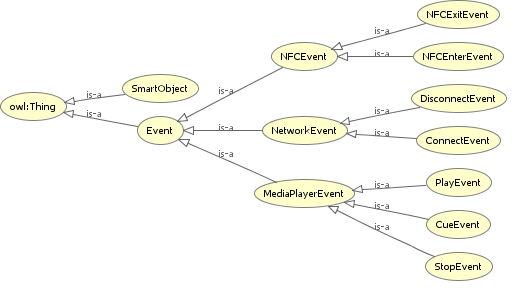
\includegraphics[width=200pt]{Ontology}
% \caption{Ontology indicating subclass relationships}
% \label{ontology1}
% \end{figure}

A first attempt at modelling the various entities in an ontology is shown in Figure \ref{ontology1}. A bottoms-up approach to modelling was used, where we attempted to model each entity using the least number of statements. These entities were later aligned with foundational ontologies -- the approach that was followed is discussed further in Chapter \ref{OntologyEngineering}. Each entity is modelled as an \texttt{owl:Class}, where all classes are subclassed from the root class, \texttt{owl:Thing}.\marginpar{The \texttt{owl:} prefix is used to denote the \ac{OWL} 2 Namespace Document located at \texttt{http://www.w3.org/2002/07/owl}.} Each edge in the graph above is a \texttt{rdf:type} relationship, and the direction of the arrow indicates the direction of the subclass relationship.

During the initial development stages, we realised that the most promising way of describing low-level interactions seemed to be to describe them in terms of \emph{interaction events}, that are defined as follows:\marginpar{Interaction events are discussed in more detail in Section \ref{InteractionEvents}.}

\begin{description}
	\item [Interaction event] An interaction event is defined as an event that occurs at a certain time instant and was generated by a specific smart object. It reports either the intent of a user's action directly, or a perceivable change in a smart object's state.
\end{description}

An interaction event in the smart space consists of an event ID, timestamp and other related information, like the smart object that generated that event. For the scenario, three types of interaction events were defined:

\begin{itemize}
	\item Network events: A \texttt{ConnectEvent} indicates that a device is entering the smart space, while a \texttt{DisconnectEvent} means that the device is exiting the smart space. 
	\item \ac{NFC} events: An \texttt{NFCEnterEvent} signifies that an \ac{NFC} tag has entered the \texttt{RFID} field, and generates a \texttt{NFCExitEvent} when it leaves the field.
	\item Media player events: When the user presses the Play button on the media player, a \texttt{PlayEvent} is generated. When the music is stopped, or at the end of the song, a \texttt{StopEvent} is generated. Pressing the Forward button forwards the song by 5 seconds. This time period is attached to a \texttt{CueEvent} using an \texttt{atTime} relationship.
\end{itemize}

The following properties were defined:\marginpar{All \ac{OWL} code listings in this thesis are written using Turtle\footnote{http://www.w3.org/TeamSubmission/turtle/} syntax. Turtle is a human-friendly alternative to \ac{XML} based syntaxes.}

\begin{minted}{turtle}
	:connectedTo
		a  owl:ObjectProperty;
	    a owl:IrreflexiveProperty;
		a owl:SymmetricProperty ;
	    rdfs:domain :SmartObject ;
	    rdfs:range :SmartObject .

	:atTime
	    a owl:DatatypeProperty ;
	    rdfs:comment "At a specific time (in milliseconds)";
	    rdfs:range xsd:integer .

	:generatedBy
	    a owl:ObjectProperty ;
	    rdfs:domain :Event ;
	    rdfs:range :SmartObject .

	:hasPosition
	    a owl:DatatypeProperty ;
	    rdfs:range xsd:integer .

	:hasRFIDTag
	    a owl:DatatypeProperty ;
	    rdfs:range xsd:string .

	:inXSDDateTime
	    a owl:DatatypeProperty ;
	    rdfs:range xsd:dateTime .
\end{minted}


The \texttt{connectedTo} object property is both \emph{symmetric} and \emph{irreflexive}. Irreflexive properties are a new feature in \ac{OWL} 2. A symmetric property is its own inverse, which means that if we indicate a \texttt{connectedTo} relationship from device A to device B, device B will also have a \texttt{connectedTo} relationship to device A. Another way to think of symmetric properties is that they are bidirectional relationships. 

An irreflexive property is a property that never relates an individual to itself \cite{Hebeler2009}. This allows us to restrict our model by not allowing a \texttt{connectedTo} relationship from a device to itself.


An example with individuals, also called instances, that make use of the ontology is shown in Figure \ref{ontologyInstance}. In the figure, classes are denoted with ellipses, individuals with boxes and datatypes as plain text. Subclass relationships are denoted with dotted lines and relationships with solid lines. It shows a Nokia N900 and N95 smartphone instantiated as \texttt{SmartObjects} with their associated \ac{RFID} tags.\marginpar{Why an \ac{RFID} tag? in Section \ref{Identification} we argue that that each smart object must be uniquely identifiable in the physical world by digital devices.}

An instantiated \texttt{NFCExitEvent}, called \texttt{event-1cecdba5}, is also shown. When an event is generated a \ac{UUID} is assigned to it, to enable the event to be uniquely identified in the smart space. It is also associated with a smart object using the \texttt{generatedBy} property. The \texttt{hasPosition} relationship provides additional metadata required by the interaction tile, which is described in the next section.  

\begin{figure}[bth]
	\digraph[scale=0.45]{ontologyInstance}{
		rankdir=LR;
		node[shape="box"];
		event1 [label="event-1cecdba5"];
		date [label="2009-12-17T13:15:16^xsd:dateTime", shape="plaintext"];
		position [label="2^xsd:integer", shape="plaintext"];
		SO [label="SmartObject", shape="ellipse"];
		Event [label="NFCExitEvent", shape="ellipse"];
		rfid1 [label="04A332D9A12580"];
		rfid2 [label="0401C4D9A12581"];
		event1 -> Event [style="dotted"];
		event1 -> date [label="inXSDDateTime"];
		event1 ->  position [label="hasPosition"];
		event1 -> NokiaN900 [label="generatedBy"];
		NokiaN900 -> AmbientLighting [label="connectedTo"];
		NokiaN900 -> rfid1 [label="hasRFIDTag"];
		NokiaN900 -> SO [style="dotted"]; 
		AmbientLighting -> NokiaN900 [label="connectedTo"];
		AmbientLighting -> rfid2 [label="hasRFIDTag"];
		AmbientLighting -> SO [style="dotted"];
	}
	\caption{Individuals that were instantiated based on the ontology}
	\label{ontologyInstance}
\end{figure}


\ac{SPARQL}\footnote{http://www.w3.org/TR/rdf-sparql-query/} is the query language for the Semantic Web. Along with \ac{OWL}, it is one of the core technologies of the Semantic Web, having been a W3C Recommendation since January 2008. \ac{SPARQL} queries are based on the idea of graph pattern matching \cite{Sequeda2012}, where data that is returned from the query is set to match the pattern.\marginpar{We also makes use of \ac{SPARQL} to define rules, which is described in Section \ref{SPIN}.}

To determine which other smart objects a specific device is connected to, a simple \ac{SPARQL} query suffices:

\begin{minted}{sparql}
SELECT DISTINCT ?object WHERE {
:deviceID :connectedTo ?object .
}
\end{minted}

\label{Jena}
A \emph{triple store} is used to store both the instances and the ontology. A triple store is a purpose-built database for storing and retrieving triples, in the format subject-predicate-object. In the above example \emph{deviceID} would be the subject, \emph{connectedTo} the predicate and \emph{?object} the object. There are a number of commercial and open-source triple store implementations. The Jena\footnote{http://jena.apache.org/} framework is a Java \ac{API} that enables access to many triple store implementations, supports \ac{SPARQL} and also has its own persistent triple store. It was used in this first implementation and was also later adopted by the \ac{SOFIA} project.

An advantage of using \ac{SPARQL} and a triple store is that it is easy to add additional constraints and/or specifics to the query, compared to a traditional \ac{SQL} database, where unions between columns and tables can get quite complicated very quickly.

To get the last event that was generated by a specific device, the \ac{SPARQL} query is a little bit more complex, but still surprisingly manageable:

\begin{minted}{sparql}
SELECT ?event ?eventType WHERE { 
:deviceID :hasRFIDTag ?tag . 
?event :hasRFIDTag ?tag .
?event a ?eventType . 
?event :inXSDDateTime ?time . 
FILTER (?eventType = :NFCEnterEvent  || ?eventType = :NFCExitEvent) 
} 
ORDER BY DESC(?time) 
\end{minted}

%Instances in the triple store could be considered to form part of the \ac{BDI} beliefs of an agent, from the \texttt{connectedTo} relationships between the smart objects, to interaction events that occurred in the past. If we describe a sequence of actions (plan) in the ontology to achieve a certain intention, we may then use the interaction events to trigger the plan, update beliefs or modify goals. Goals may be defined in the ontology as desires, where we can add the necessary property restrictions to ensure that active desires are consistent. If sequences of actions are sufficiently defined in the ontology, we may even be able to use a reasoner to infer subsumption hierarchies of plans based on the user's current actions, which in turn would allow us to determine the user's intentions.

How do we model the semantic connections between devices? Since semantic modelling is property-oriented instead of object-oriented, we started by focusing on the possible predicates that can be used to describe connections. We need a way to model whether a connection is possible --- this can be done with a \texttt{canConnectTo} property. We also need to know if a device is currently connected to another device --- \texttt{connectedTo}. Then we need a way to model the capabilities that each device provides. In this first iteration, we defined two properties called \texttt{consumes} and \texttt{provides}. They are used as follows:

\begin{minted}{turtle}
	NokiaN900 provides AudioCapability .
	NokiaN95 consumes AudioCapability .
\end{minted}

During the later design iterations we decided to model capabilities as functionalities of a device instead, and make the name of the property clearer to indicate whether it is a functionality of a source or a sink. The property \texttt{provides} was changed to \texttt{functionalitySource}, and \texttt{consumes} was changed to \texttt{functionalitySink}. These early properties are mentioned here for the sake of completeness, and to show how aspects of the ontology have changed between iterations.

% \begin{tabular}{cc}
% 	Iteration 1 (08/09) & Final iteration \\
% 	canConnect & canConnectTo \\
% 	isConnected & connectedTo \\
% 	provides & functionalitySource \\
% 	consumes & functionalitySink \\
% \end{tabular}


\section{Device design}
\label{DeviceDesign1}

Based on the scenario, a number of smart objects had to be constructed or repurposed, and the necessary software had to be developed.

To explore the different possibilities of visualising and manipulating connections between devices, a number of different prototypes were constructed. The first of these is called the \emph{interaction tile}. 

%- Components used: Interaction Tile, Lamp
%- 5800 (\euro 265) as cheap phone with WiFi


\subsection{Interaction Tile}

\begin{figure}[bth]
\centering
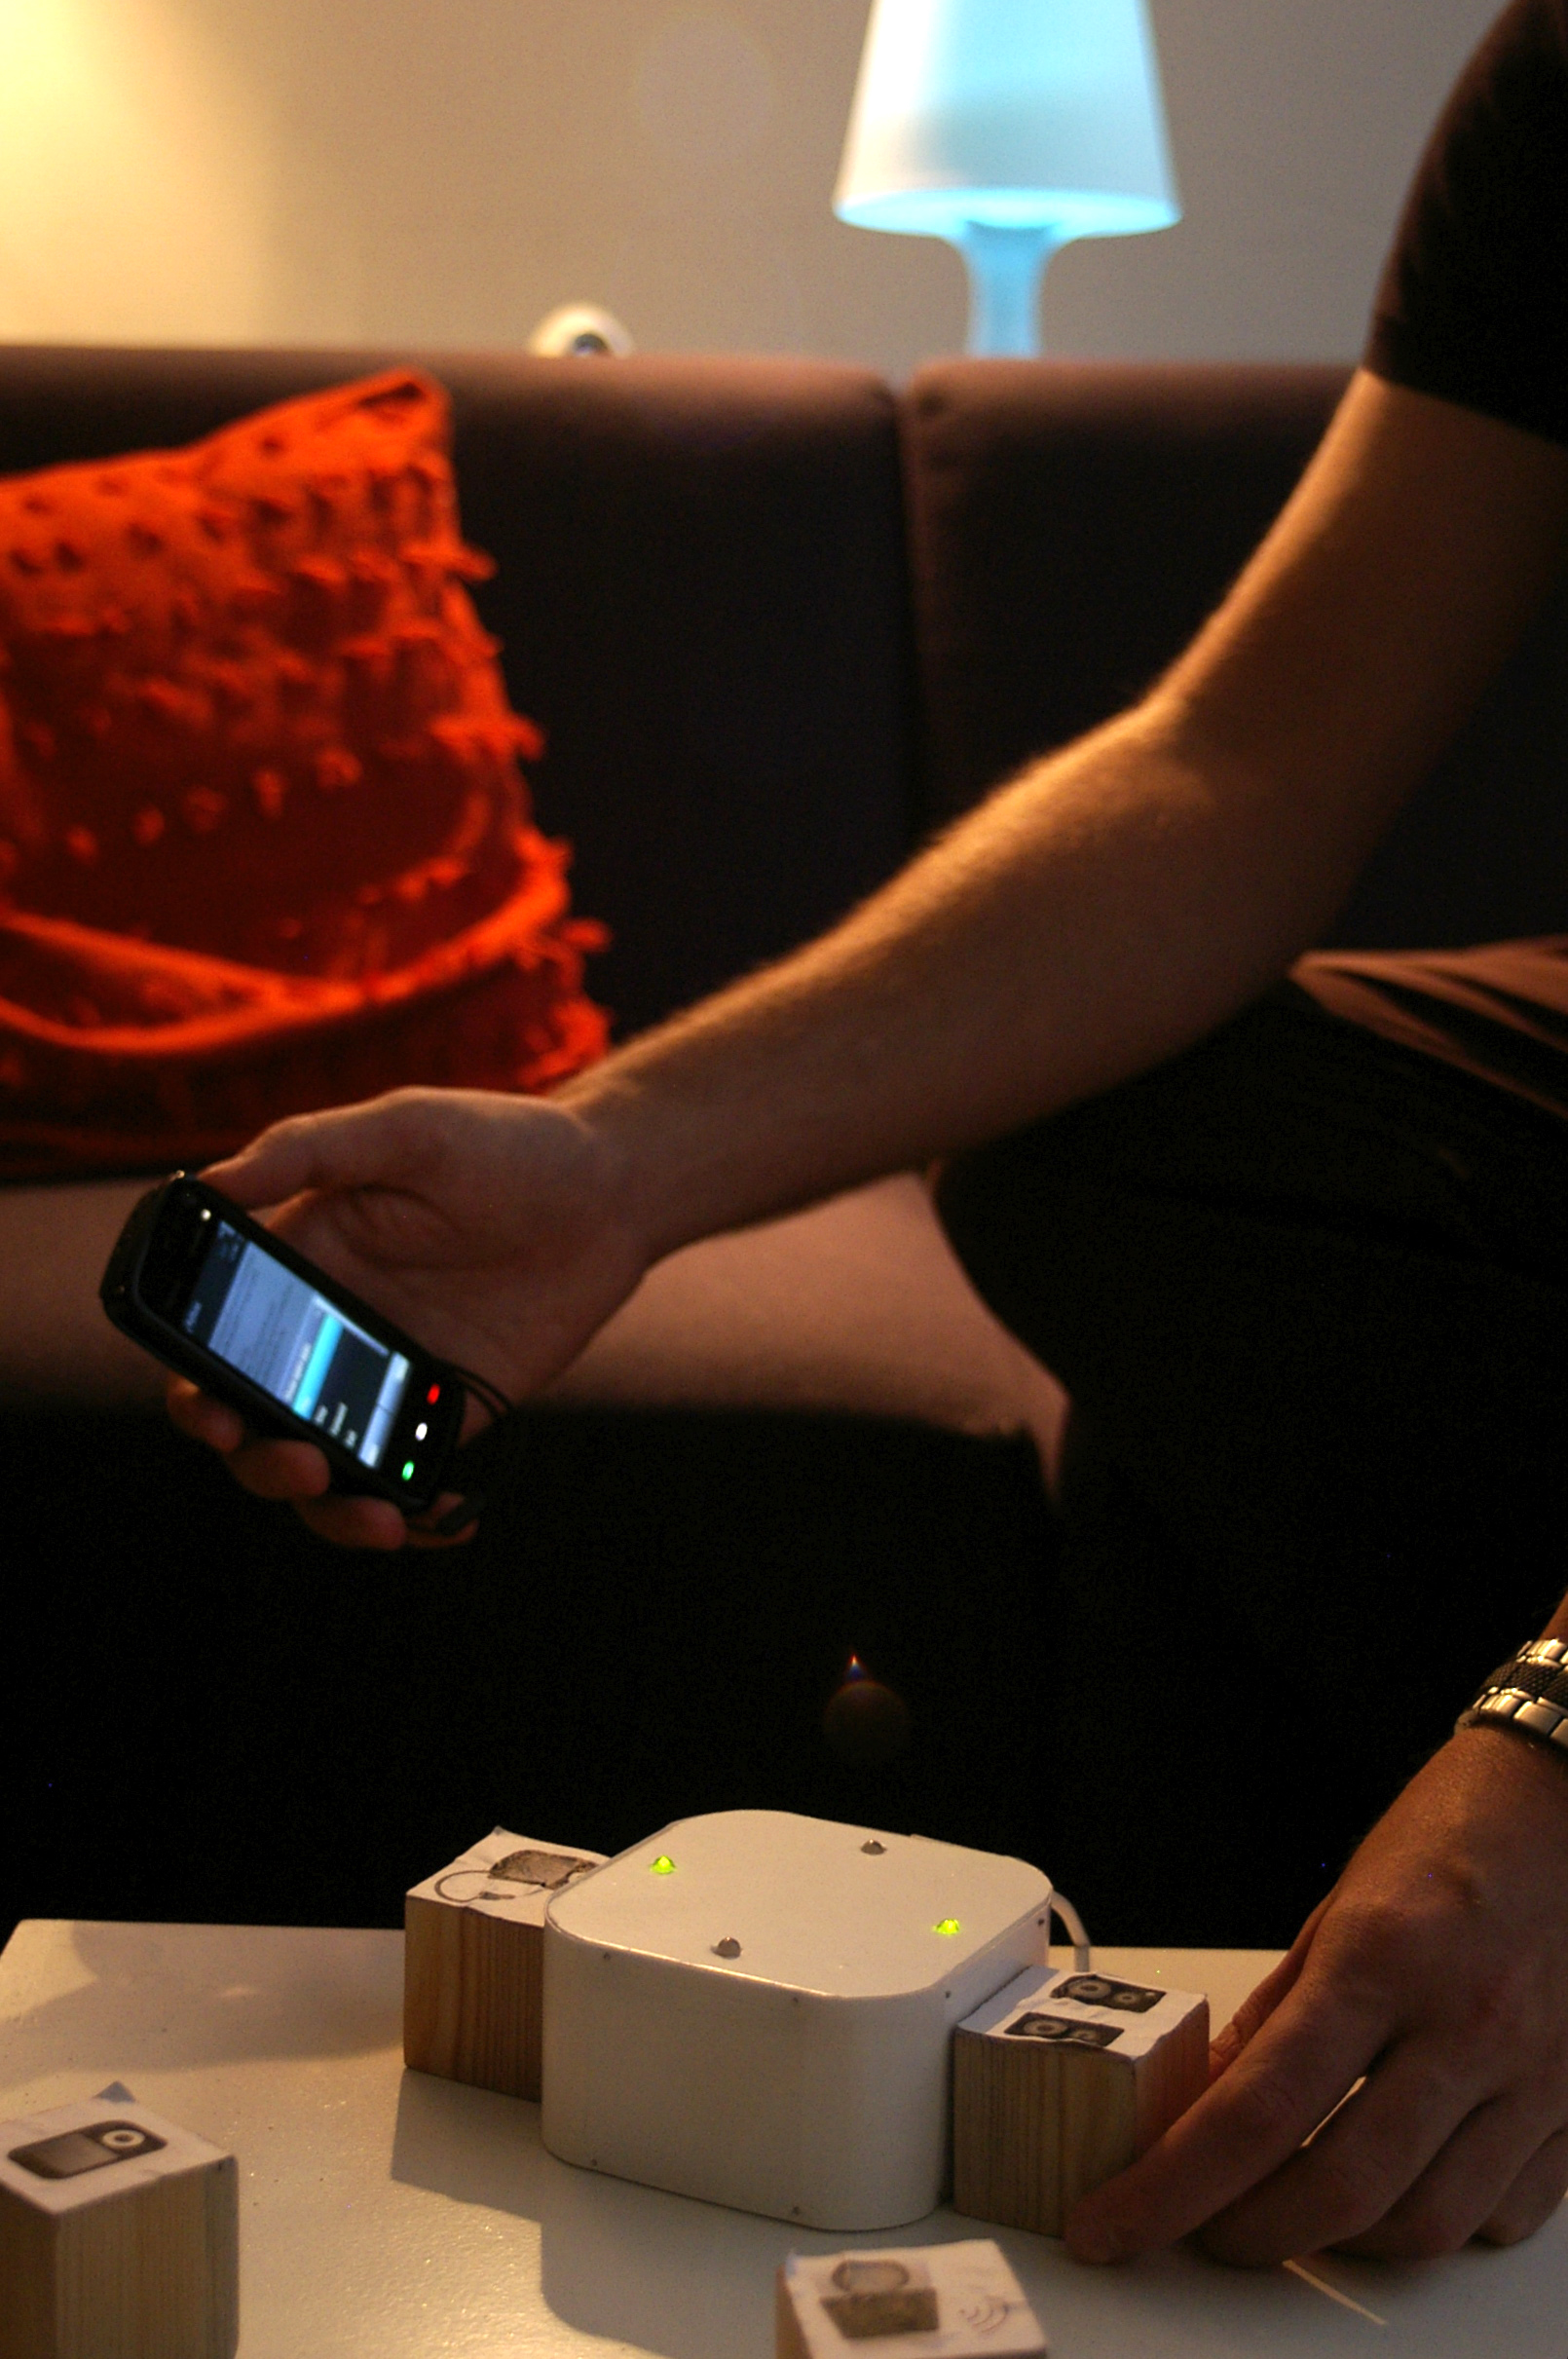
\includegraphics[width=260pt]{tile1}
\caption{The interaction tile and mobile phone}
\label{tile1}
\end{figure}

The interaction tile, shown in Figure \ref{tile1}, was inspired by Kalanithi and Merrill's ``Siftables'' cubes \cite{Merrill2007}. It was designed to explore and manipulate connections through direct manipulation -- by making simple spatial arrangements. Each device in the smart environment is represented by a cube containing an \ac{RFID} tag and a small magnet, with an icon on the top of the cube to signify the device being represented. When a cube is placed next to one of the four sides of the tile, an LED on the tile lights up to indicate that it has been recognised. When a second cube is placed next to the tile, the following LED visualisations are used:

\begin{itemize}
	\item Pulsating green light - a connection is possible
	\item Constant green light - a connection exists
	\item Red light - no connection is possible
\end{itemize}  

The interaction tile visualises the various connections by allowing a user to explore which objects are currently connected, and what connections are possible. By means of putting a cube representing a device close to one of the four sides of the tile, a user can check if there is a connection, and if not, whether a connection is possible. By shaking the tile it is possible to create a connection between two devices, or where there is an existing connection, to break the connection. The interaction tile consists of the following components:

\begin{itemize}
	\item Arduino 
	\item ACR122/Touchatag 13.56MHz \ac{RFID} reader
	\item Multi-colour LEDs
	\item Accelerometer
	\item Vibration motor
	\item Piezoelectric speaker
	\item magnetic switches
\end{itemize}

The Arduino communicates with a PC via a serial interface over USB, while the \ac{RFID} reader uses \ac{PC/SC} drivers over USB.\marginpar{The \ac{RFID} reader component has been tested under Windows, Linux and Mac OS X.} The accelerometer is used to measure when the user is shaking the tile, while the vibration motor and speaker provide haptic and auditory feedback. The magnetic switches are used to determine which side of the tile a cube has been placed. The final laser-cut version of the interaction tile prototype is shown in Figure \ref{tile2}.

\begin{figure}[bth]
\centering
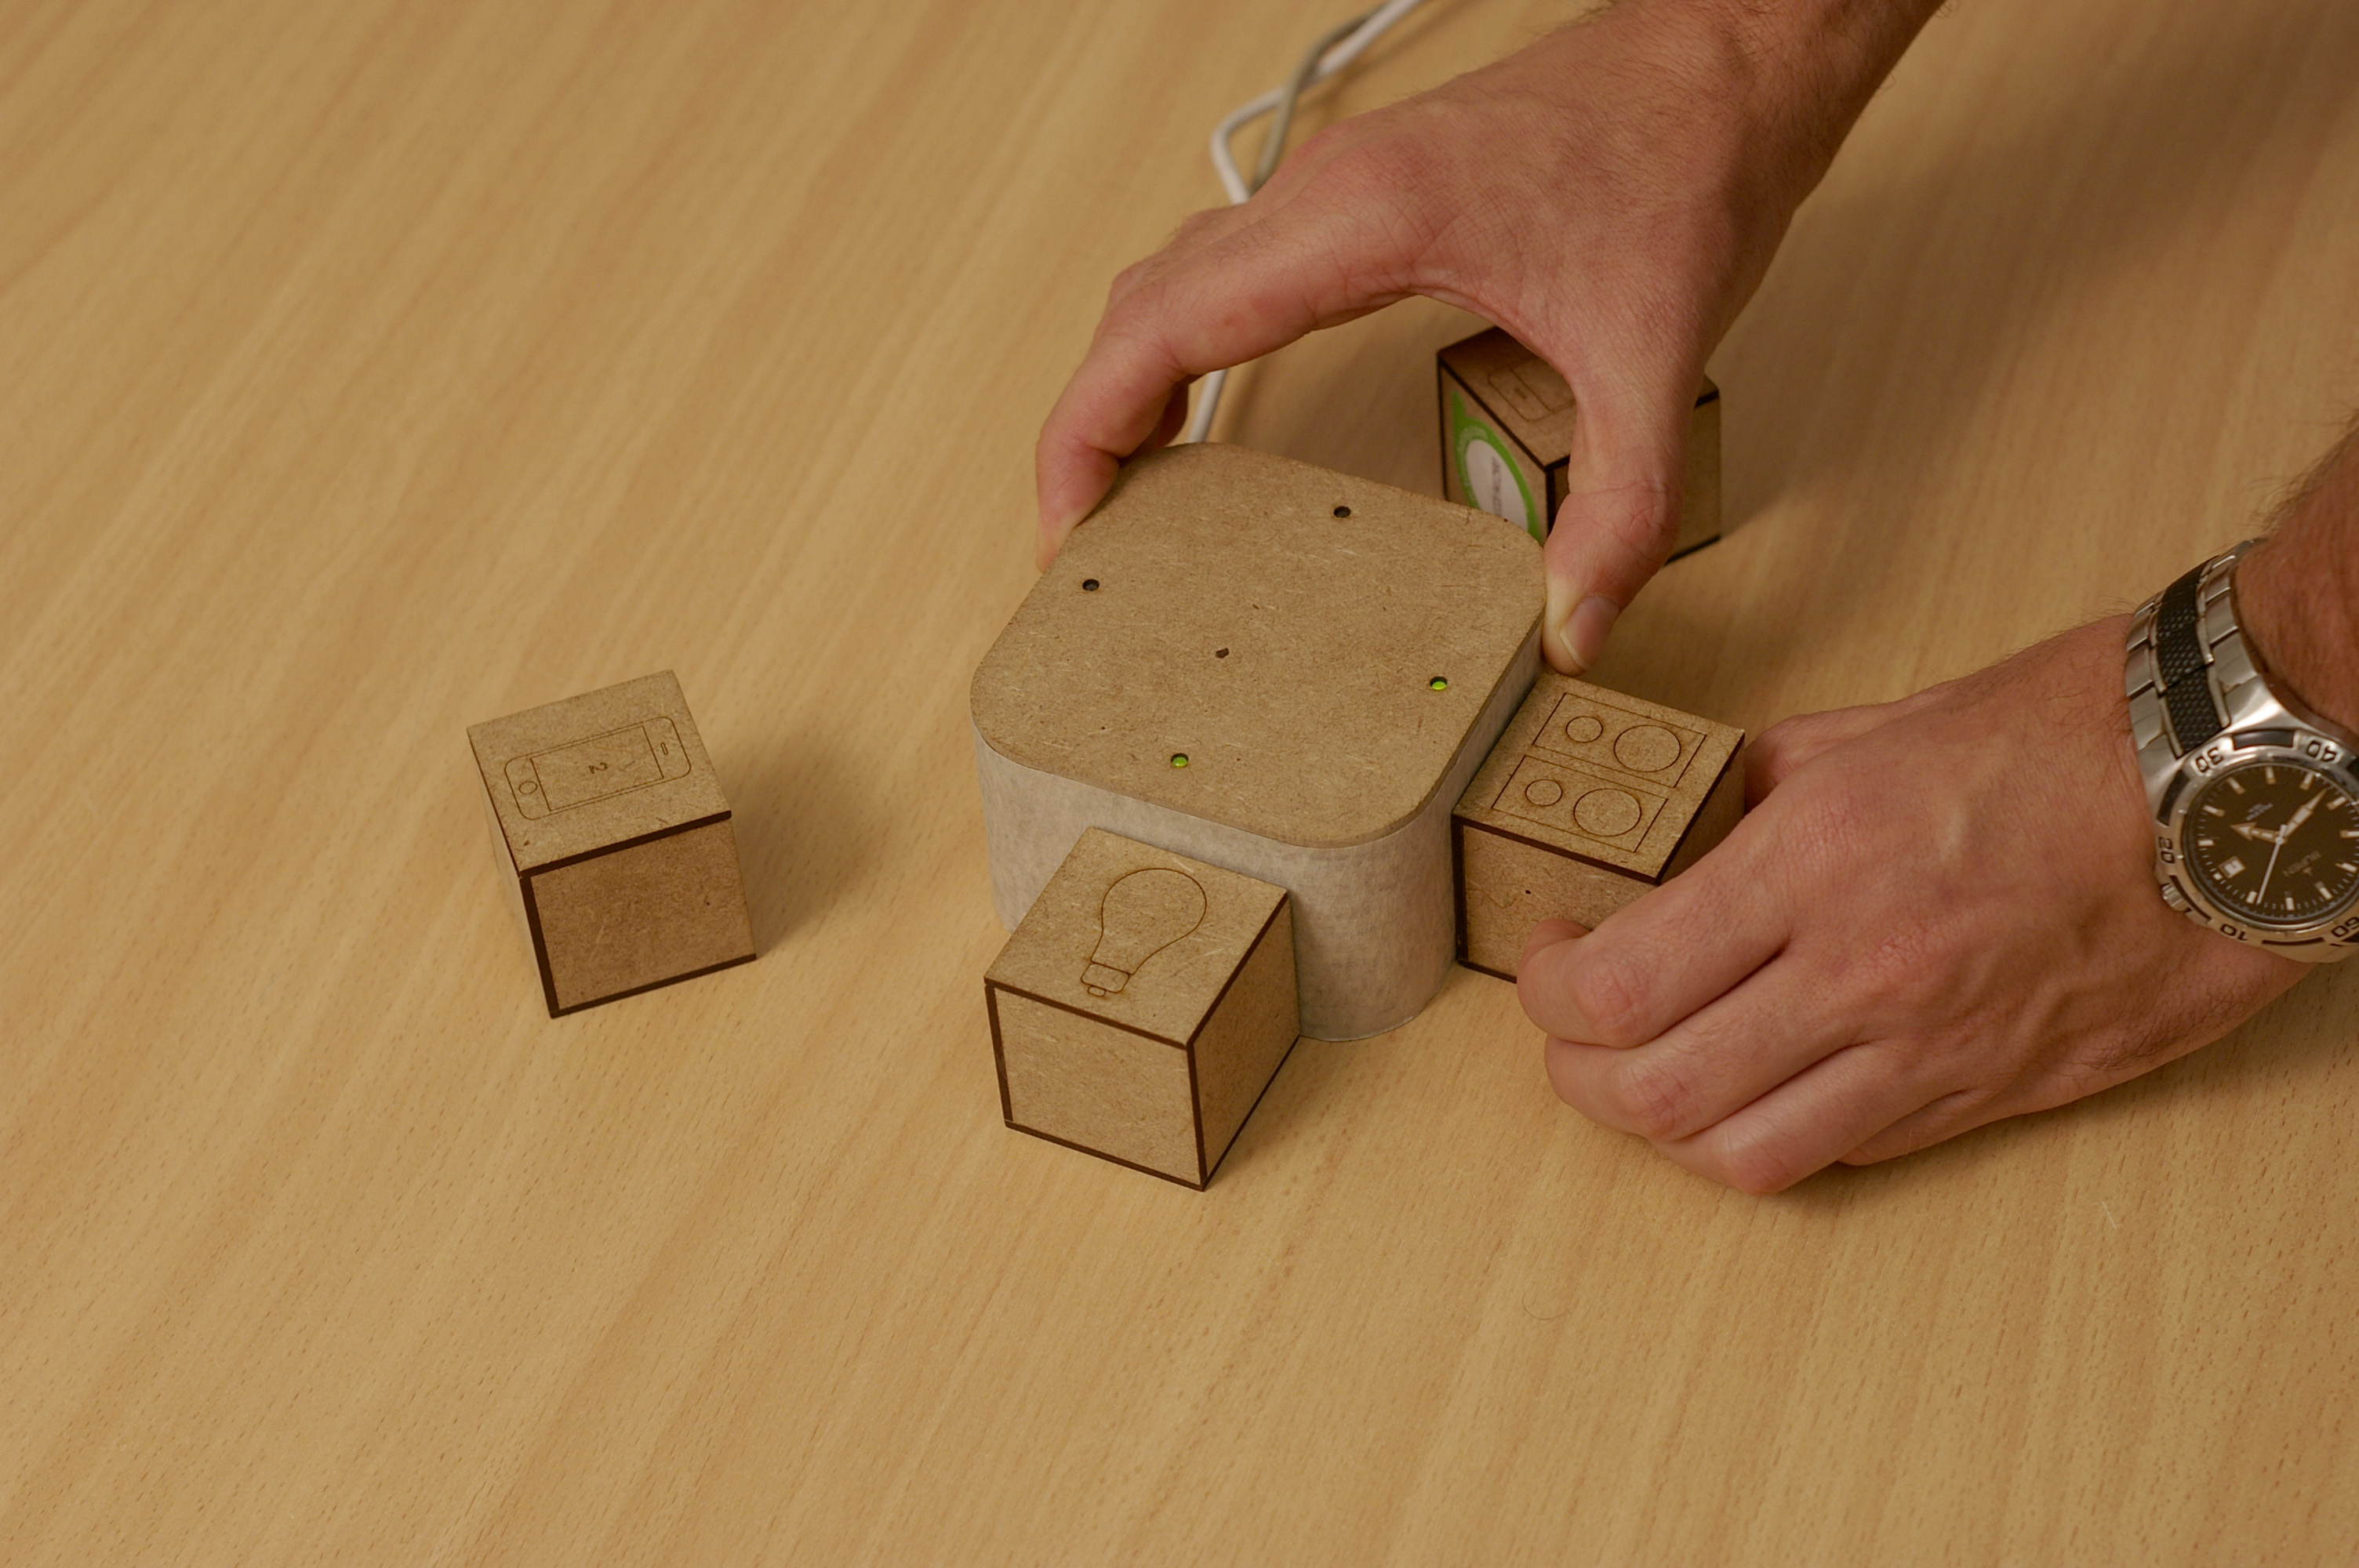
\includegraphics[width=260pt]{tile2}
\caption{A laser-cut version of the interaction tile prototype}
\label{tile2}
\end{figure}

Two alternative designs are presented in Van der Vlist's thesis \cite{Bram}. A more detailed discussion of the interaction tile and how its design is informed by product semantics is available in \cite{VanderVlist2010}. 

\subsection{Lamp}
\label{Lamp}
To create the ambient lighting system, we replaced the internals of a table lamp with an RGB LED array and an Arduino\footnote{ http://www.arkadian.eu/pages/219/arduino-controlled-ikea-lamp}. A Bluetooth module was connected to the Arduino to facilitate communication with a computer, the final result of which can be seen in Figure \ref{lamptile}.\marginpar{The Ikea Lampan lamp that was used for the prototype currently retails for around \euro 3.} 

\begin{figure}[bth]
\centering
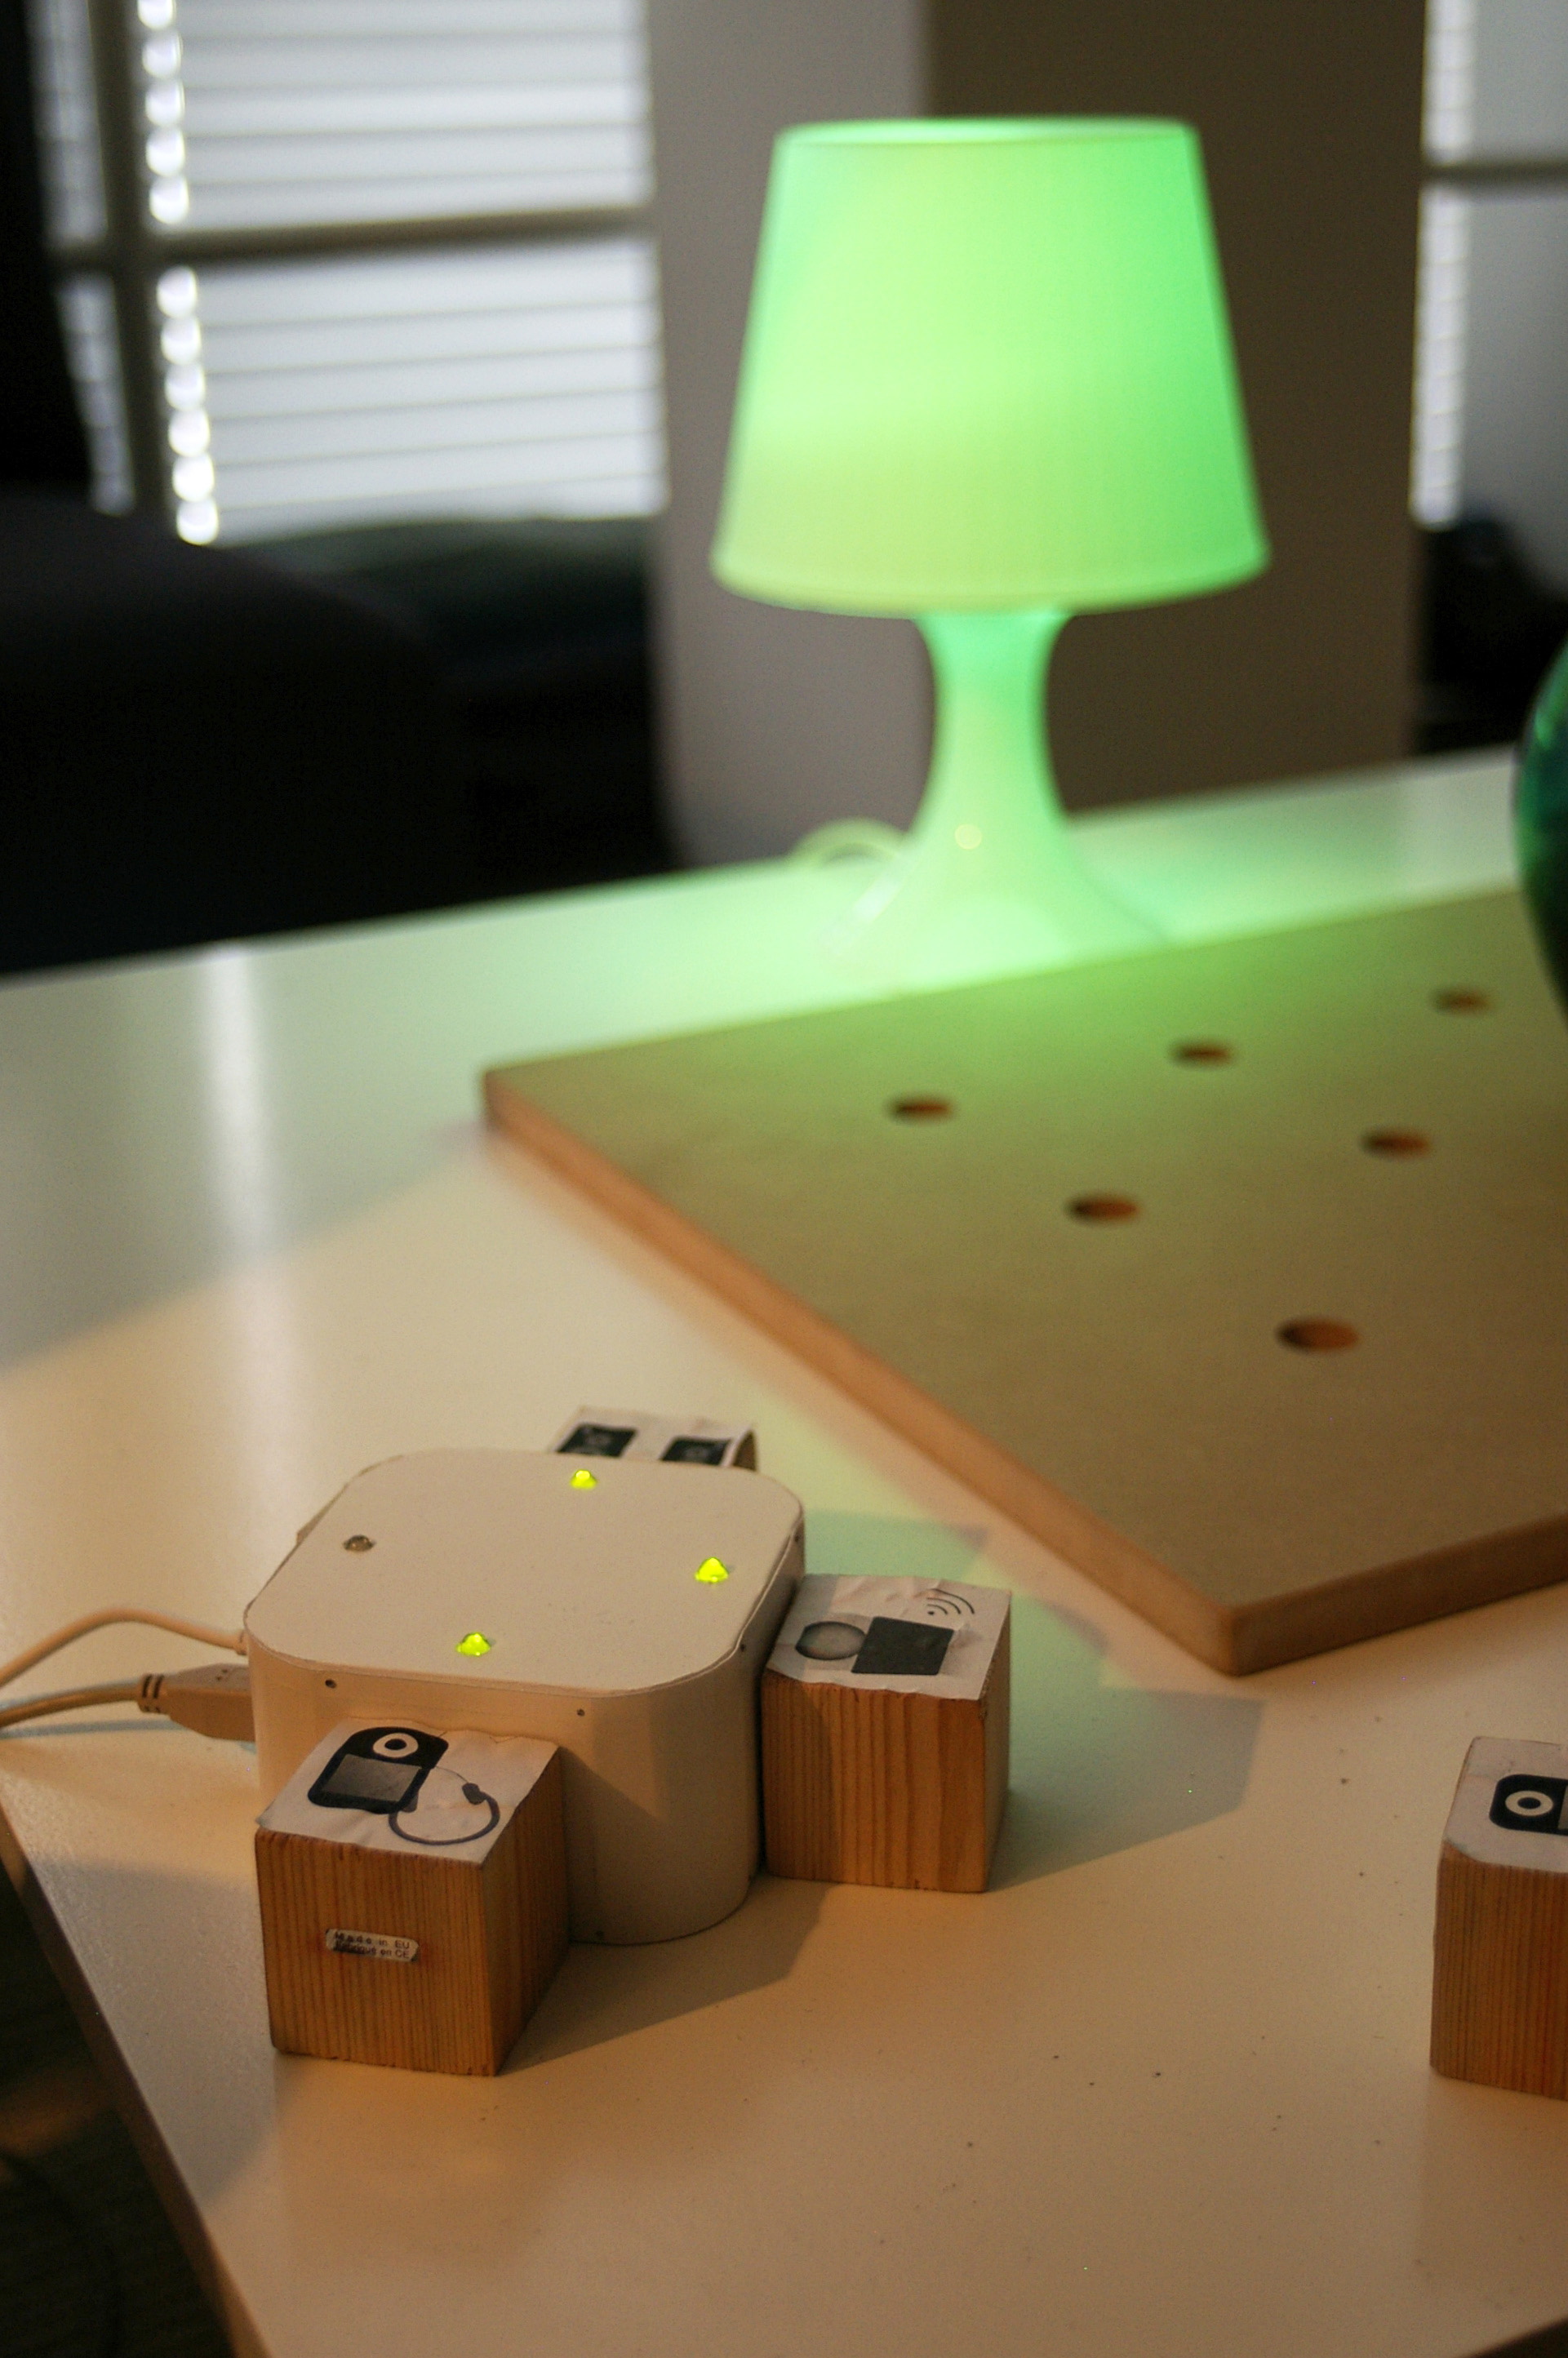
\includegraphics[width=260pt]{lamptile}
\caption{The interaction and cubes, with the lamp in the background}
\label{lamptile}
\end{figure}

The coloured lighting can be changed by sending three RGB values (in the range 0-255) to the lamp via the serial-over-Bluetooth interface.

\subsection{Mobile phones}

For the first iteration, a Nokia N95 and Nokia 5800 XpressMusic phone (shown in Figure \ref{lampphone}) was used. The two phones use the Symbian S60 operating system, and Python for S60 was used to write software for the mobile phones.\marginpar{Python for S60 is Nokia's port of the Python programming language for Symbian devices.}

\begin{figure}[bth]
\centering
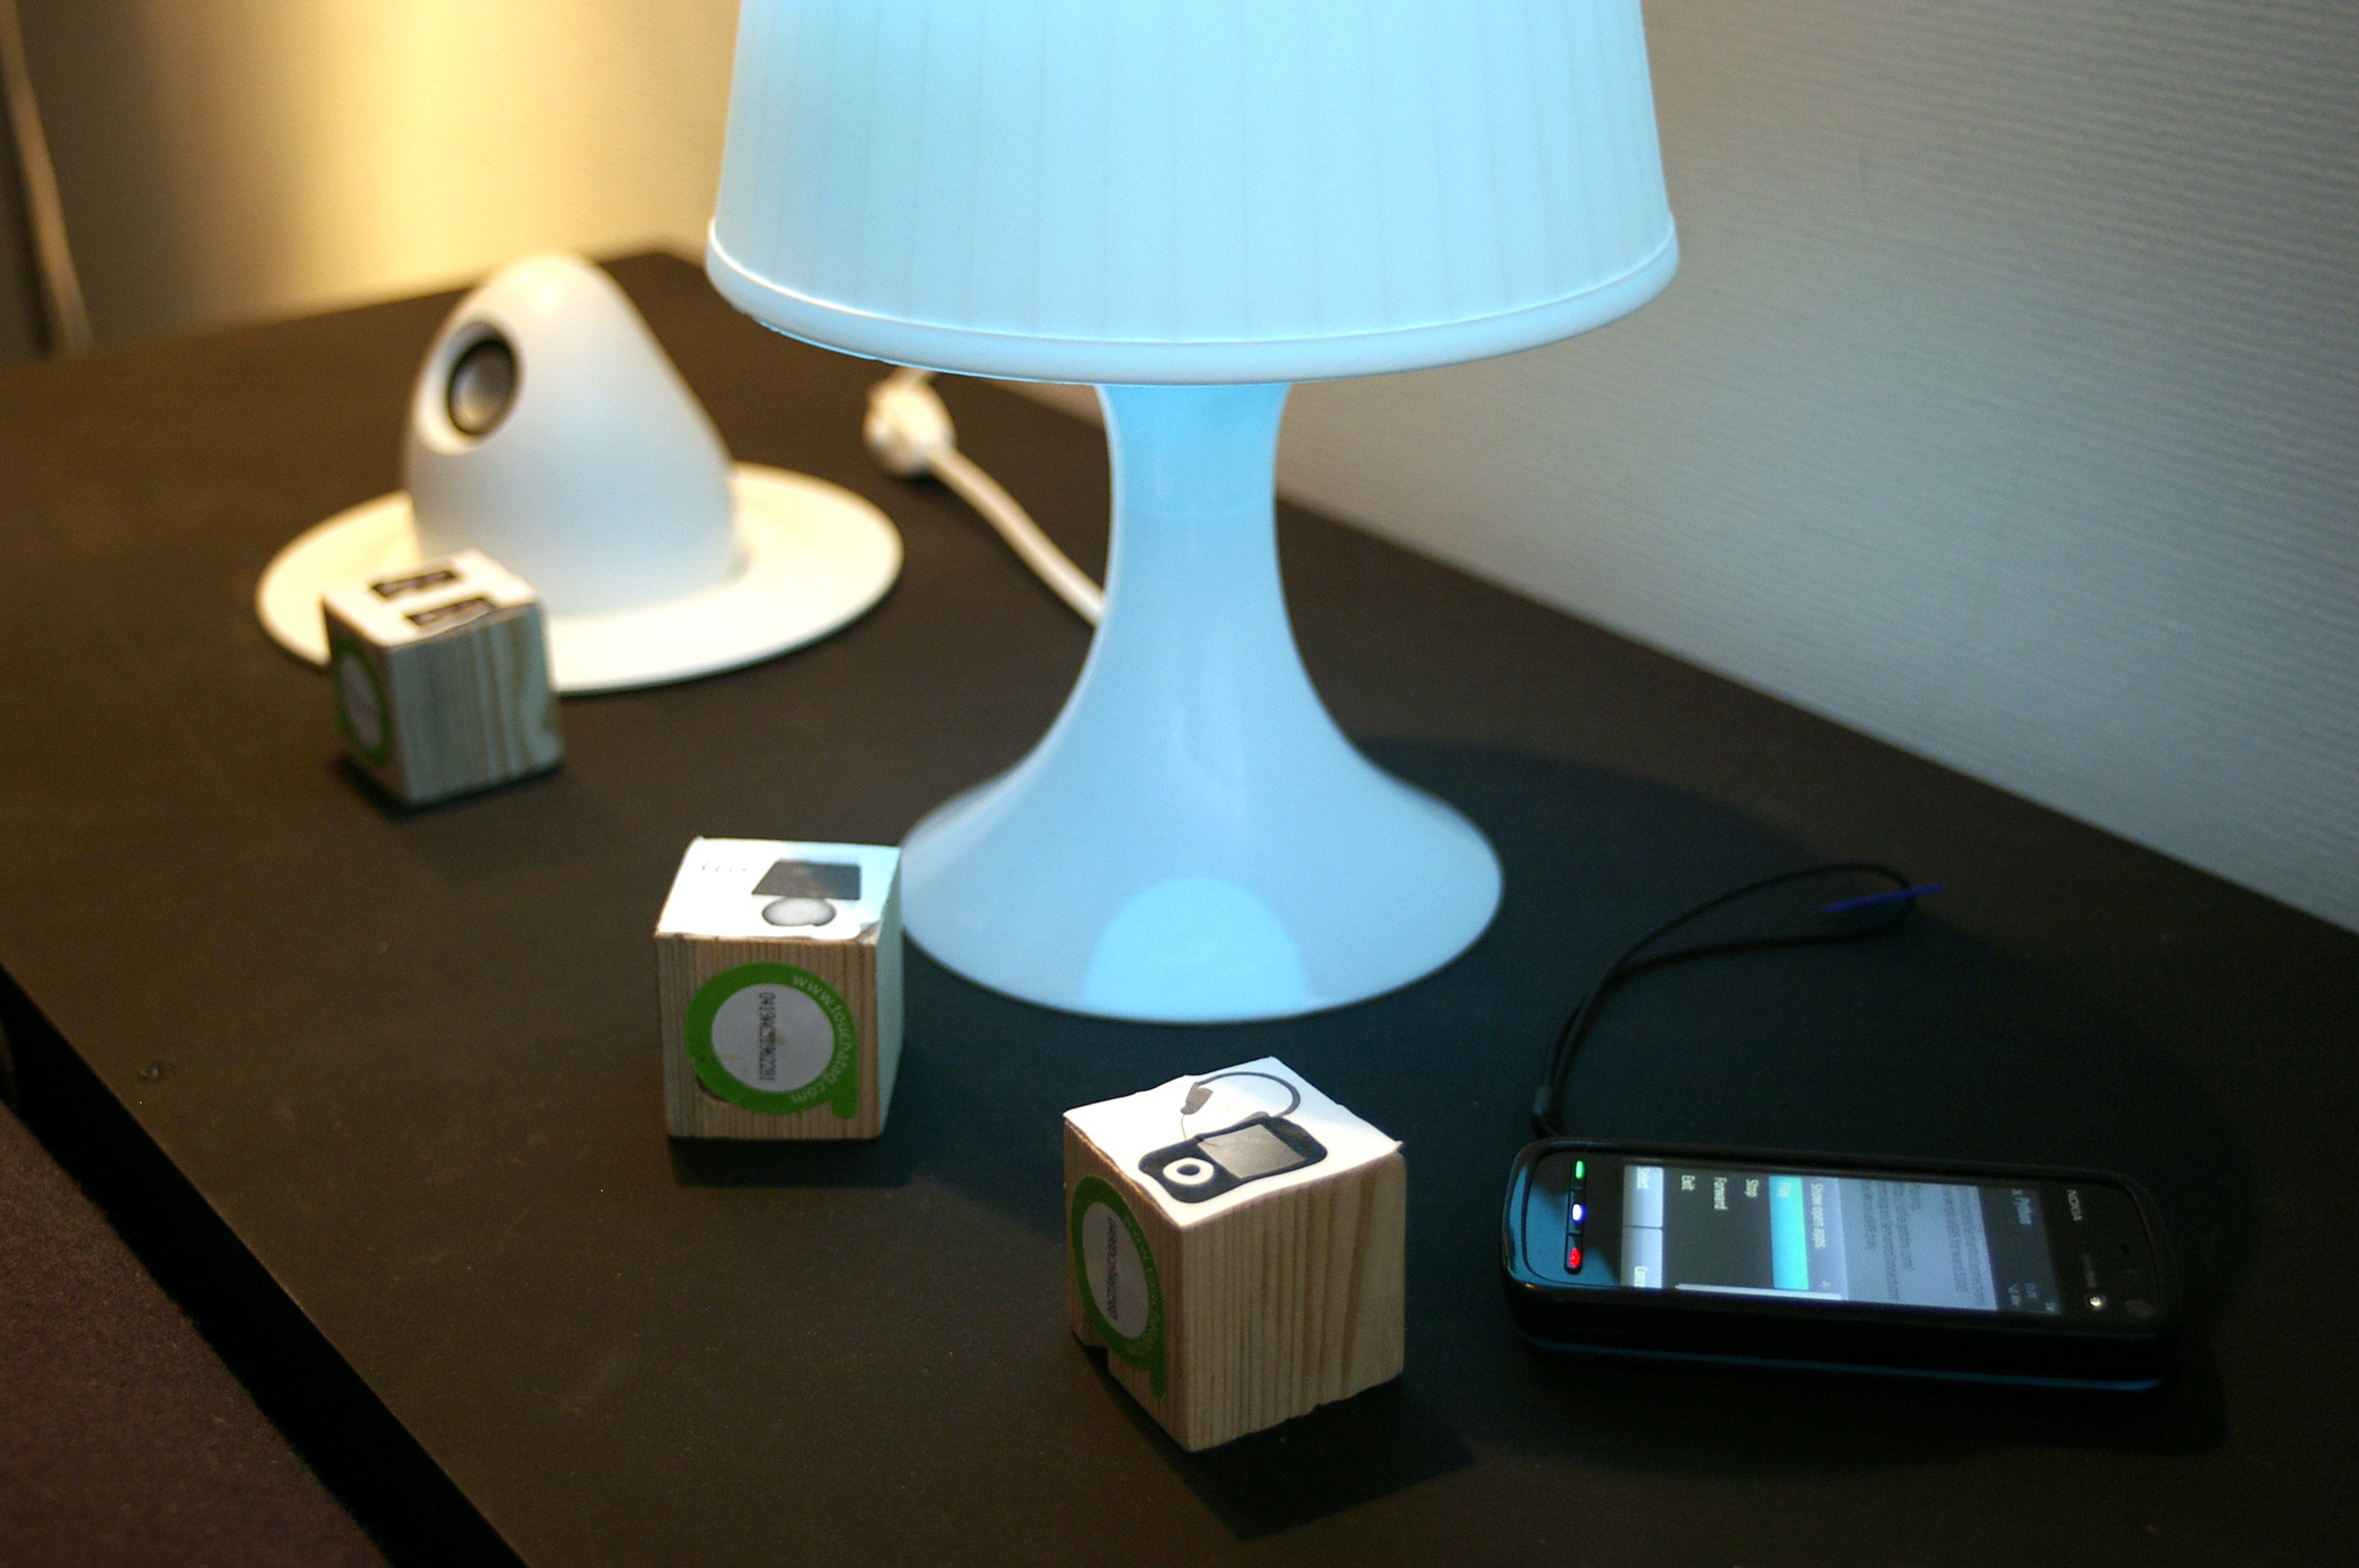
\includegraphics[width=260pt]{lampphone}
\caption{The Nokia 5800 XpressMusic mobile phone with the lamp and some cubes}
\label{lampphone}
\end{figure}



\section{Implementation}

\begin{figure}[bth]
\centering
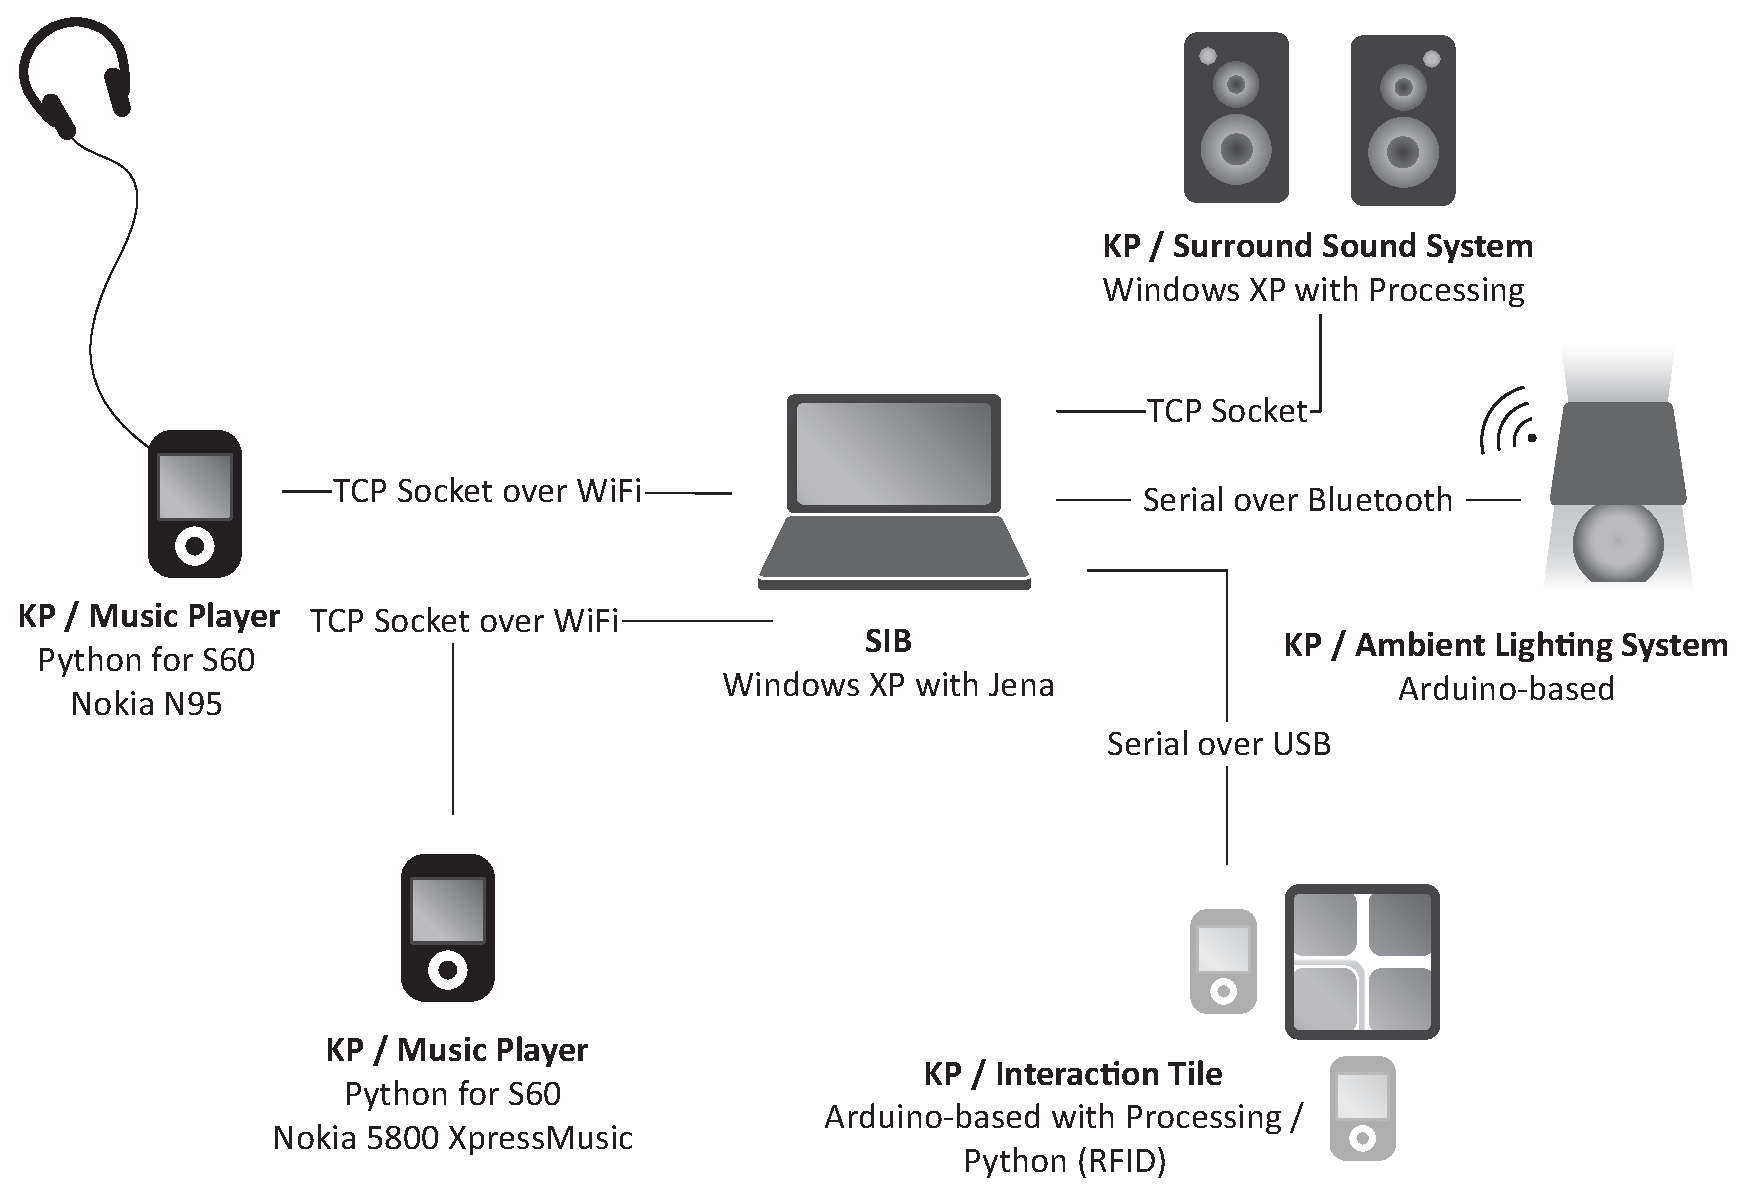
\includegraphics[width=360pt]{SemanticConnections.eps}
\caption{An overview of the demonstrator}
\label{semanticConnections}
\end{figure}

Following the design and development of the ontology and required devices, a demonstrator that implements the the scenario was created. A visual overview of the demonstrator can be seen in Figure \ref{semanticConnections}. A video of the scenario is available\footnote{https://vimeo.com/15594590}.

\begin{figure}[bth]
\centering
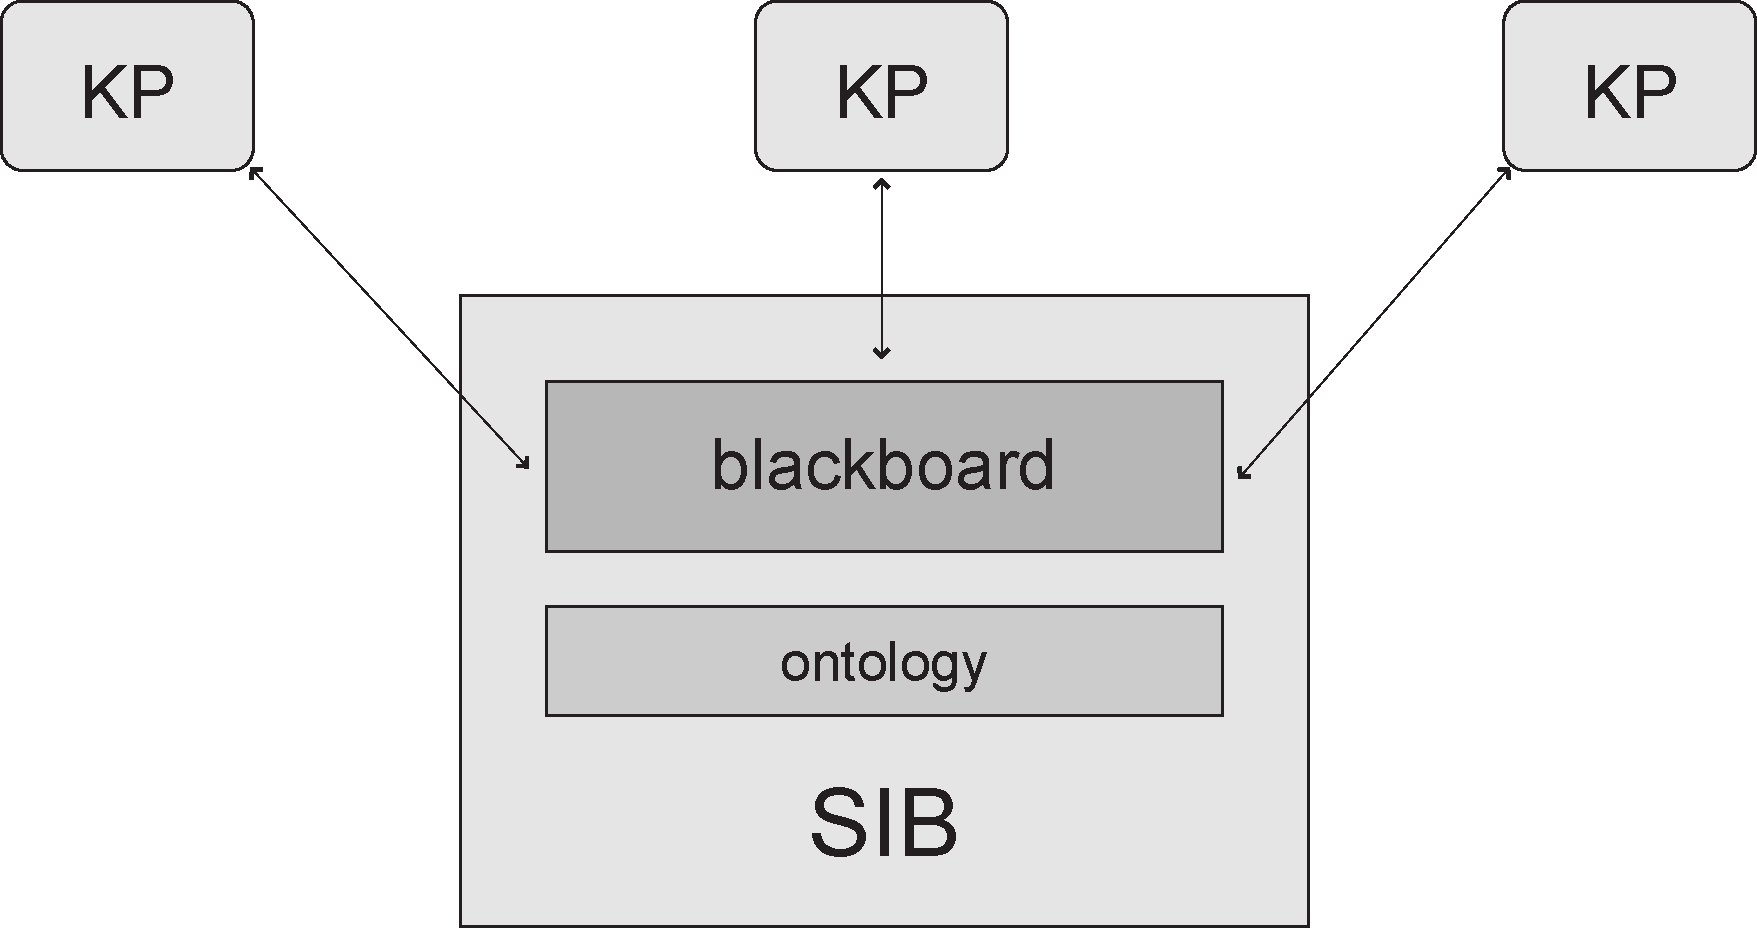
\includegraphics[width=260pt]{blackboard}
\caption{System architecture of demonstrator}
\label{blackboard}
\end{figure}

Each device in the demonstrator is represented by a \ac{KP} software module. \acp{KP} communicate via the \ac{SIB}, as shown in Figure \ref{blackboard}. As discussed in Section \ref{sofia}, the \ac{SIB} acts as an information broker, distributing messages between devices. This was an early design decision to reduce coupling, by minimising direct communication between devices, with all messages relayed via the \ac{SIB}. This philosophy of having a blackboard architectural model, where devices can write to and read from, was followed through all subsequent design iterations. The technical implementation of the various \acp{KP} are described in the following subsections.\marginpar{The system architecture model is described in more detail in Chapter \ref{SoftwareArchitecture}.}


\subsection{Interaction Tile KP}

The interaction tile \ac{KP} was written in Python and tested on Ubuntu Linux 10.04. On startup, the \ac{KP} connects to the Arduino inside the interaction tile via the serial-over-USB interface. It established a connection with the \ac{SIB}, after which it connects to the \ac{RFID} reader inside the tile.\marginpar{The open-source rfidiot.org library was used to communicate with the \ac{RFID} reader.}

The \ac{KP} then enters an event loop, waiting until a cube is placed next to the tile. When this happens, the Arduino sends the position of the cube next to the tile to the \ac{KP} via the serial interface. The \ac{RFID} tag is read, and a \texttt{NFCEnterEvent} is generated. After the \ac{RFID} tag is read it is temporarily disabled, to ensure that the tag will only be read again after being removed from the field and coming into range again.

If the tile is shaken and a connection is possible, the \ac{KP} updates the \ac{SIB} by inserting \texttt{connectedTo} relationships between the devices, represented by the cubes next to the tile. If there are existing connections, the \texttt{connectedTo} relationships are removed instead. When a cube is removed from the tile, the Arduino again send the position of the cube via the serial interface to notify the \ac{KP}. The \texttt{python-pyscard}, \texttt{pcsc-tools} and \texttt{pcscd} \ac{PC/SC} libraries are required on Ubuntu Linux to communicate with \ac{RFID} reader.

\subsection{Music Player KP}
\label{MusicPlayerKP}
This Python-based \ac{KP} runs on Symbian S60. It has been tested on a Nokia N95 and Nokia 5800 XpressMusic phone. When the \ac{KP} starts up, it connects to the \ac{SIB}, generates a \texttt{ConnectEvent} and subscribes to new \texttt{PlayEvent}s, \texttt{StopEvent}s and \texttt{CueEvent}s. It then enters an event loop. Pressing the play/stop/forward buttons on the phone's \ac{GUI} will generate the corresponding event, and the \ac{KP} will also respond to events generated by other devices that it is connected to via the \texttt{connectedTo} relationship.

Another version of the music player \ac{KP} was developed for a Nokia N900 smartphone that runs on Maemo 5 Linux. This \ac{KP} was also written in Python and makes use of the PyQt4 library. This \ac{KP} is functionally equivalent to the Symbian S60 version, apart from running on the Maemo platform and using the Qt4 Phonon framework to provide music play/stop/forward capabilities.
% - N900 - used pyside and QtMobility (24/08/10)

\subsubsection{Light KP}

This \ac{KP} was written in Java and makes use of the Minim audio library\footnote{http://code.compartmental.net/tools/minim/} for beat detection, in order to generate meaningful lighting patterns that can be sent to the table lamp.\marginpar{The Minim audio library is part of the Processing software development environment, used for interaction design prototyping.}

The \ac{KP} listens for media player events from connected devices, and generates RGB values based on the rhythm of the music. These RGB values are then sent to the Arduino in the table lamp via the serial-over-Bluetooth interface. On Ubuntu Linux the \texttt{librxtx-java} package is required for serial communication when using Java.

%- Use ~/code/semanticconnections/docs to describe technical implementation 
%	- C-based SIB (Piglet triple store, with component requirements 19/05/10 - to appendix?)
%	- dependencies (06/09/10)

\subsubsection{SIB}
%- Components required are (18/05/10 Notebook1)

The first \ac{SIB} implementation used in the \ac{SOFIA} project is called Smart-M3, developed by Nokia, and an open source implementation is available online\footnote{http://sourceforge.net/projects/smart-m3/}. The \ac{SIB} is written in C and uses Nokia's Piglet triple store as a database backend. It is only available on Linux as it makes of the D-Bus message bus system. Other dependencies include the Avahi service discovery framework and Expat XML parser.  The \ac{SIB} consists of a daemon called \texttt{sibd}, which communicates with \acp{KP} over TCP/IP using a \texttt{sib-tcp} connector module.  


\section{Discussion \& Conclusion}

%- Proximal interactions with tangible interfaces
%- First use of Smart-M3
%- Triple-format queries from KP e.g. None,ie:hasRFIDTag,None (Evaluate against SPARQL queries from KP?)
%- Input: Interaction events (multimodal fusion) and implicit interaction (sensor observations) (discussed in TiiS paper)



This first iteration constructed a number of devices that could be reused in future iterations, and explored approaches to creating connections between devices. These approaches were focused at proximal interactions with tangible interfaces instead of the usual \ac{GUI}-based solutions. Let us look at some issues that were uncovered during the implementation, followed by a conclusion. 

Most of the \ac{RFID} readers and tags targeted at the amateur and hobbyist markets, like the PhidgetRFID and Innovations ID-12 modules, operate in the 125KHz range. While they are relatively cheap and readily available, the 125KHz readers cannot read multiple tags within range of the reader at the same time. For this a 13.56MHz reader is required. The most widely used \ac{RFID} tags at the moment, the MiFare range owned by NXP, operate at 13.56MHz. These tags are used in most public transport payment systems, including the London Oyster Card and the Dutch OV-Chipkaart system.

A relatively cheap 13.56MHz \ac{RFID} reader system, the ACR122, is developed by Hong Kong-based \ac{ACS}. It uses the NXP PN532 chip to read \ac{RFID} tags. \marginpar{A rebranded version of the ACR122, called the Touchatag\footnote{http://www.touchatag.com/}, is currently sold with 10 tags for around \euro 30.} The reader has an onboard PCB antenna -- to extend the range of the unit we removed two capacitors on the PCB and soldered in an external ANT-1356M coil antenna from RF Solutions.
%- Hacking the Touchatag (\euro 33) by adding our own external antenna (see circuit diagram)

This iteration details the first use of Smart-M3, where \acp{KP} communicate with a \ac{SIB} using \ac{SSAP}\cite{Honkola2010}. \ac{SSAP} consists of a number of operations to insert, update and subscribe to information in the SIB. These operations are encoded using XML. A triple-format query from a \ac{KP} is sent, and the response from the \ac{SIB} is in triple-format as well. %An example of a triple-format query is \mint{turtle}|None hasRFIDTag None| where \texttt{None} is used to denote the wildcards in the query. The response to this query would be a list of triples containing smart objects and their associated \ac{RFID} tags.

We attempt to solve the interoperability problem by following a blackboard-based approach. Some of the problems associated with current blackboard-based platforms are scalability and access rights. While the goals of this thesis do not involve solving these problems, they should be considered as possible constraints. In Chapter \ref{Evaluation} we will look in more detail at the performance-related issues of the system architecture. 

The evaluation of this iteration, where the various alternative tangible approaches are compared in a usability study, is discussed in more detail in \cite{Kwak2011}. This study was performed in the Context Lab at the Eindhoven University of Technology, and made use of the Teach-Back protocol \cite{VanDerVeer2003} and Norman's Action Cycle Diagram \cite{Norman1998}.




%(already in intro)
% We consider context awareness to be one of the most important features of a smart environment, especially when we consider a user's interaction with the smart space. Considering the parallel nature of our interaction with the physical world, any smart space will require context to help it make sense of the many different ways in which users map their tasks onto the environment.
% 
% Where the system tries to predict what the user is trying to accomplish, by being adaptive and anticipatory, we need to identify ways to give the users appropriate means to express themselves. The possibilities, available services and information that exist in the smart environment needs to be communicated in a meaningful way. Only if this is done correctly will users be able to build helpful mental models of the functionality the environment has to offer, set goals and make plans on how to act. By developing novel and meaningful interaction devices, the user can then perform the necessary actions and the system can in turn try to understand the user's goals and make the match to its internal models. We see a vital role here for the theory of \emph{product semantics} \cite{feijs-commutative}, the study of how artefacts acquire their meaning and use its theories to define common concepts and semantics. 

%To be able to create a personalized environment, we consider both runtime task models and the BDI model to be important. Task models may be used to describe the user's actions, while the BDI model may be used to represent the psychological, social and situational aspects of the tasks. Once the task model is defined, the system can adapt to the user, by mapping the user's current activity or task to higher-level goals and intentions.

%The BDI model approach focuses on the anticipatory aspect of ambient intelligence, where the system tries to predict what the user is trying to accomplish. We also hope to use the low-level events and command currently implemented in the system to automatically infer higher-level tasks and goals, with the final step being able to model the user's (and/or agent's) intentions using an ontology.

%end SISS2010